%
% Appendix C - Additional Screenshots
%
\chapter{Additional Screenshots} \label{app:screenshots}

This appendix gives full-size screenshots referenced from Chapter~\ref{cap:frontend} but not shown inline there, to keep that chapter within the report's page budget.

\section{Calendar Views} \label{app:calendar-views}

Referenced from Section~\ref{sec:frontend-calendar-ui}. The Month view is shown inline as Figure~\ref{fig:calendar}; the remaining four are given here in full size.

\begin{figure}[htbp]
\begin{center}
\resizebox{\textwidth}{!}{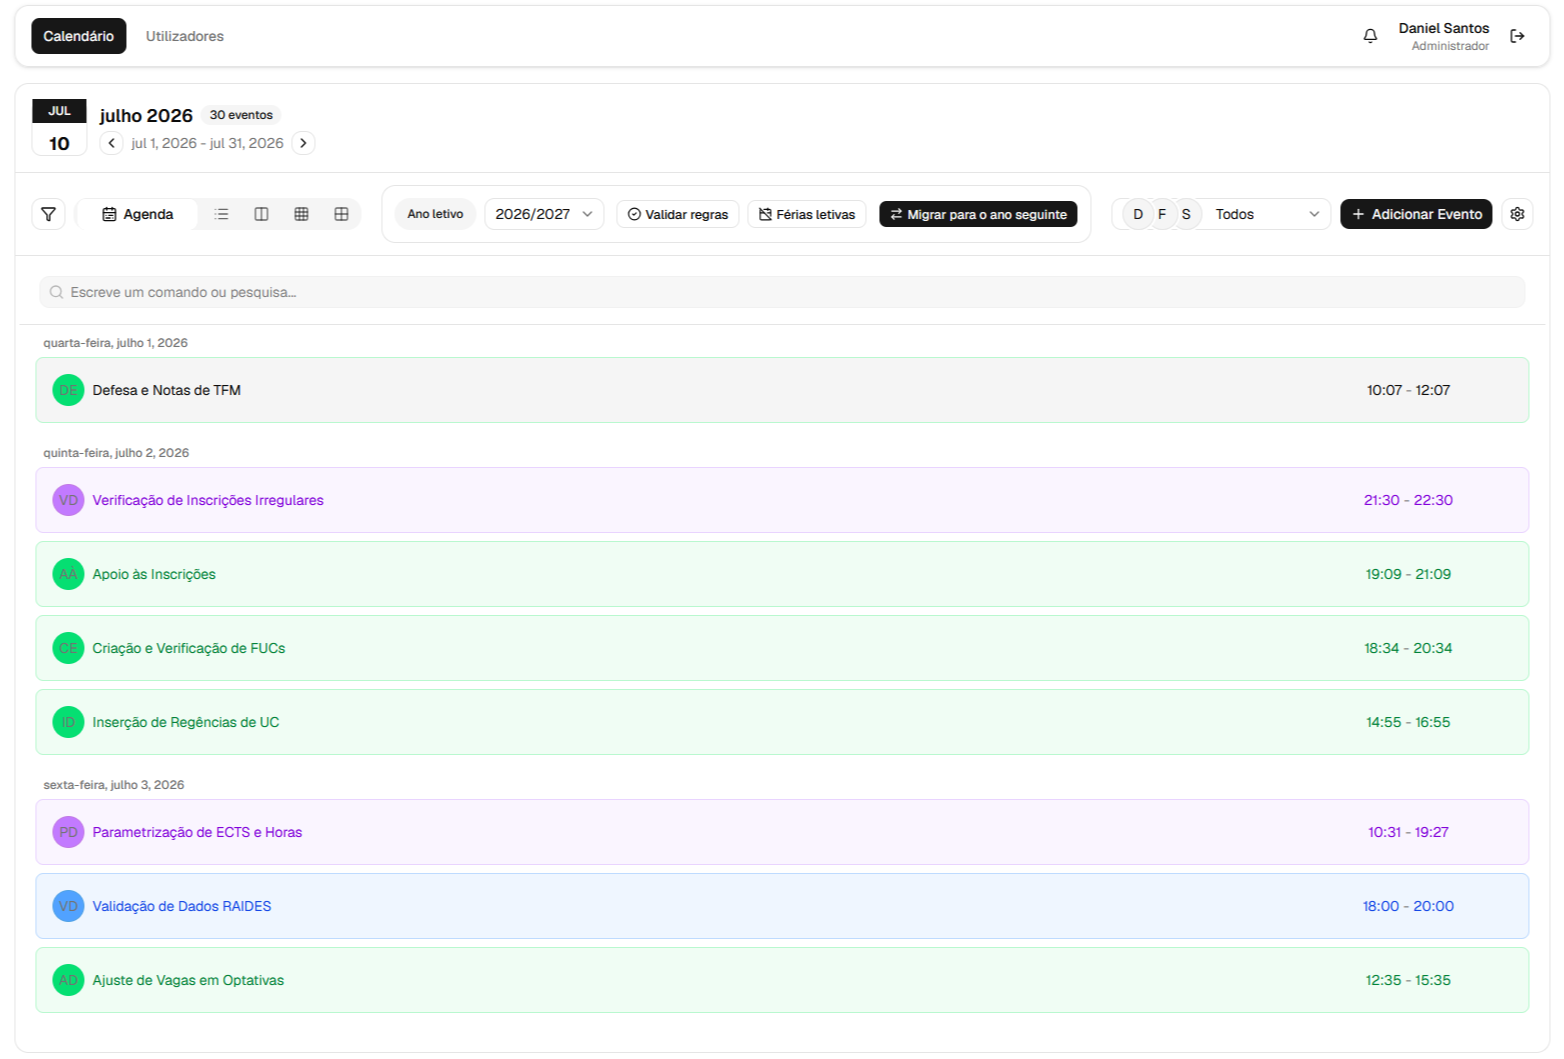
\includegraphics{./figures/app_screenshots/calendar_View_agenda.png}}
\end{center}
\caption{Calendar interface, Agenda view: a scrollable list of occurrences grouped by date or category.}\label{fig:calendar-agenda}
\end{figure}

\clearpage
\begin{figure}[htbp]
\begin{center}
\resizebox{\textwidth}{!}{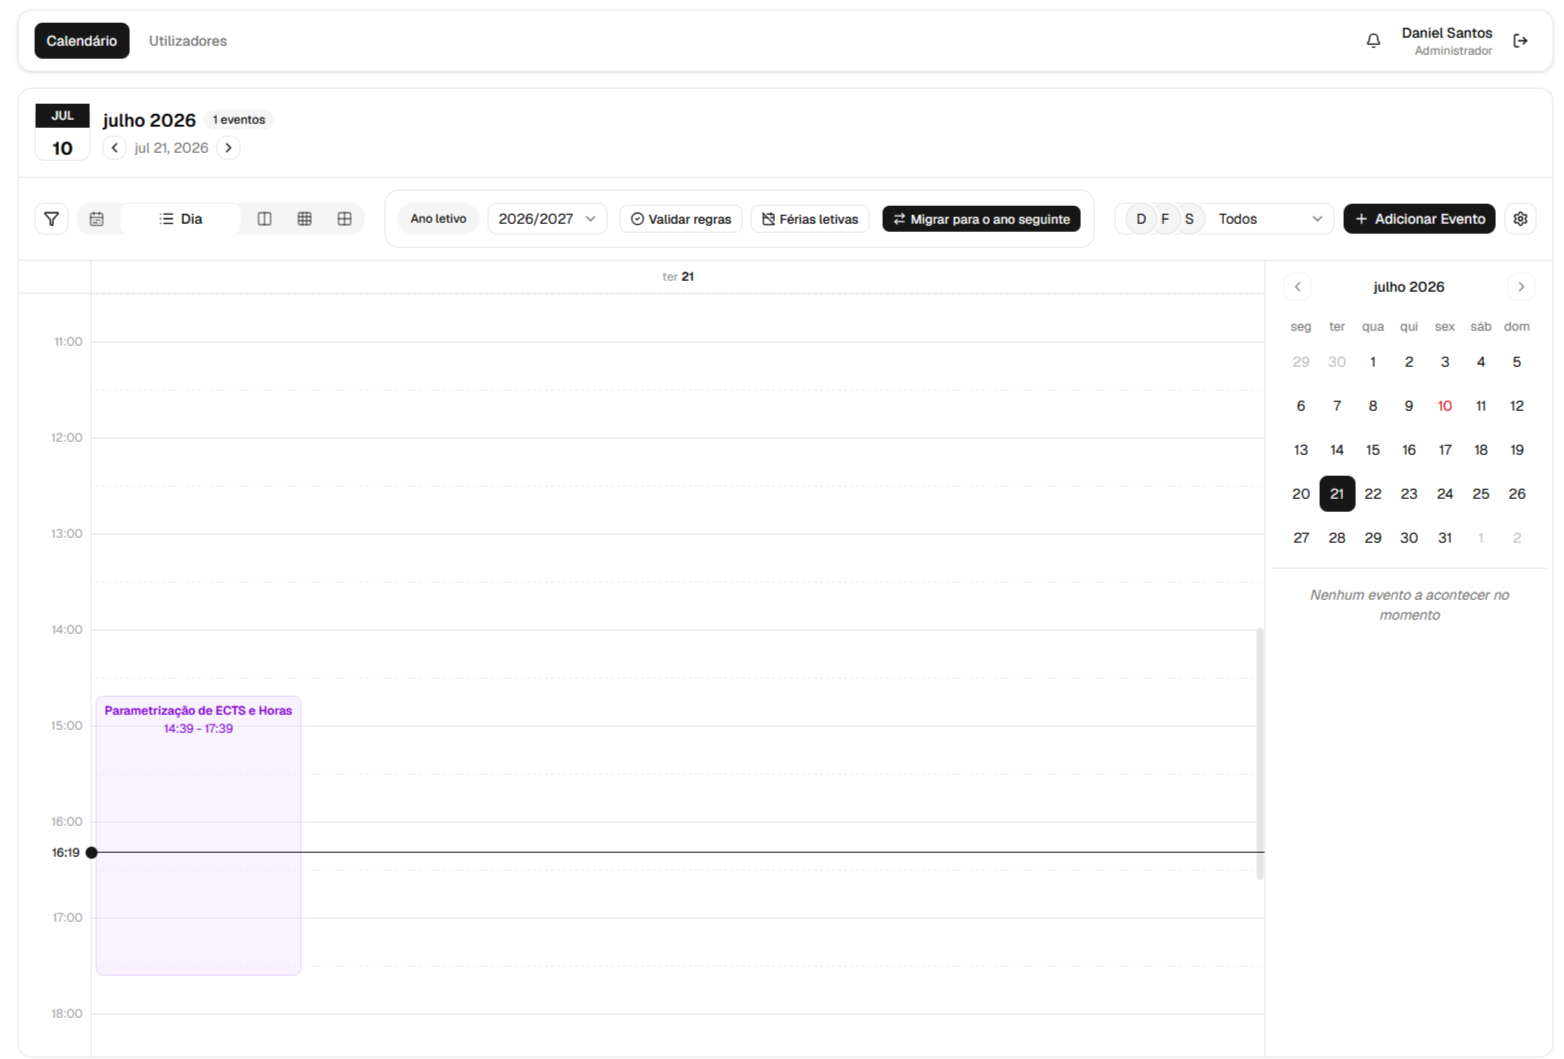
\includegraphics{./figures/app_screenshots/calendar_View_day.png}}
\end{center}
\caption{Calendar interface, Day view: a single-day time grid supporting drag-and-drop rescheduling and resizing.}\label{fig:calendar-day}
\end{figure}

\clearpage
\begin{figure}[htbp]
\begin{center}
\resizebox{\textwidth}{!}{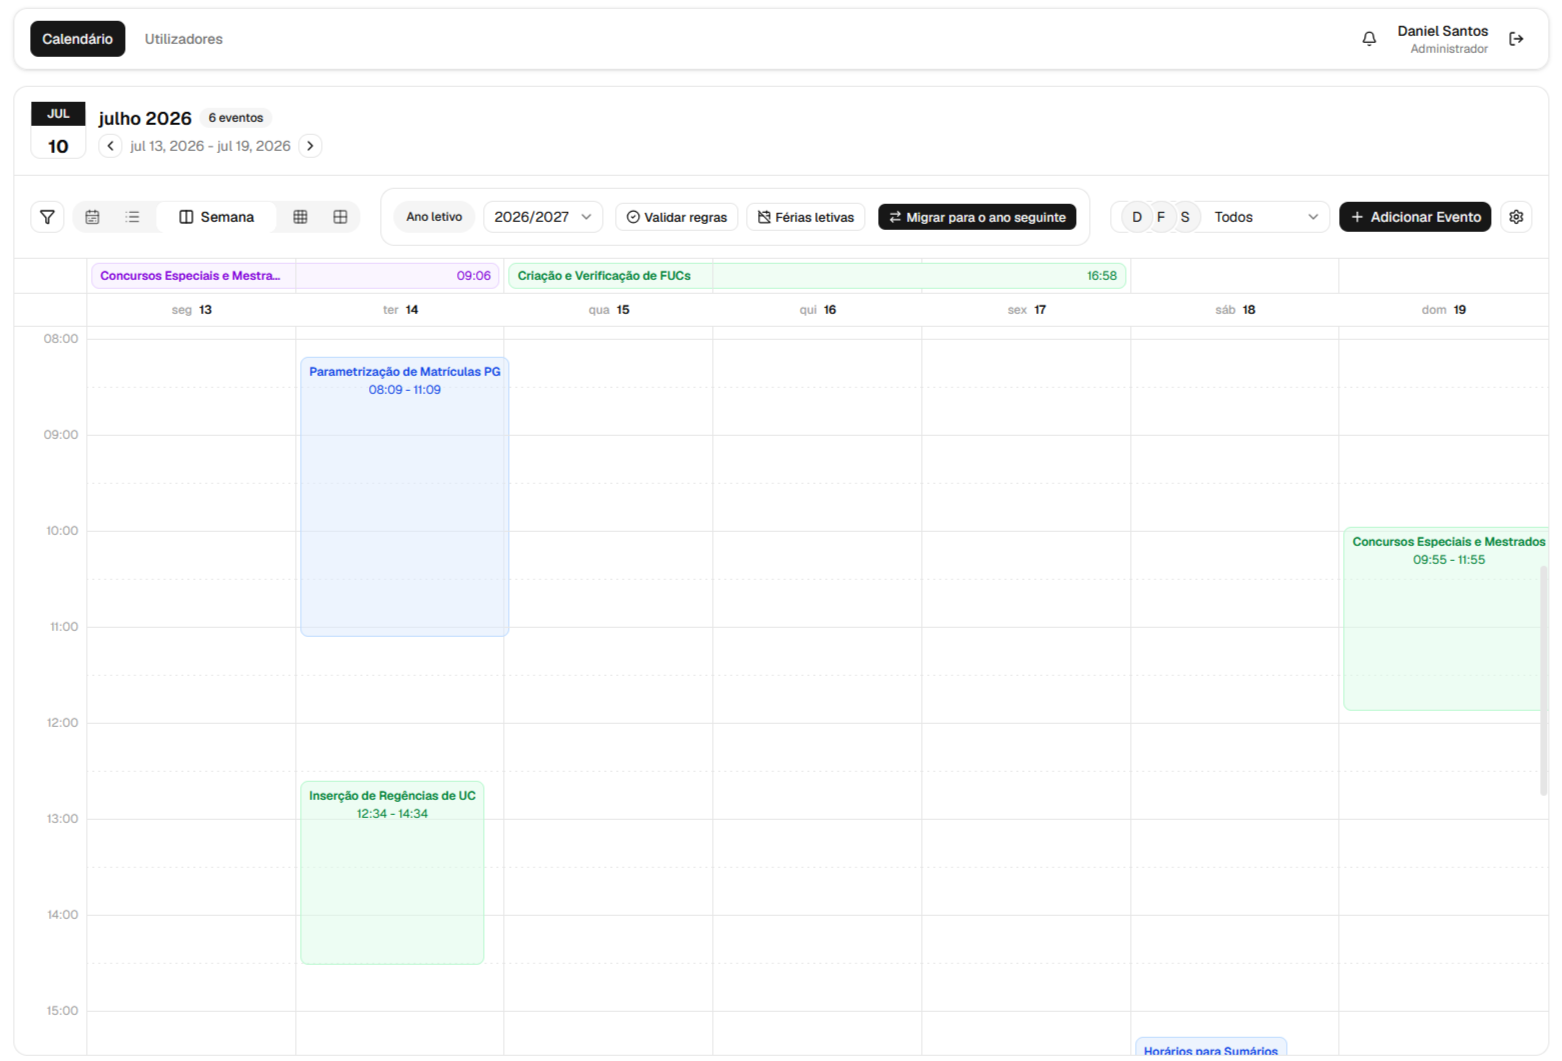
\includegraphics{./figures/app_screenshots/calendar_View_week.png}}
\end{center}
\caption{Calendar interface, Week view: the same time-grid interactions as the Day view, spanning a full week.}\label{fig:calendar-week}
\end{figure}

\clearpage
\begin{figure}[htbp]
\begin{center}
\resizebox{\textwidth}{!}{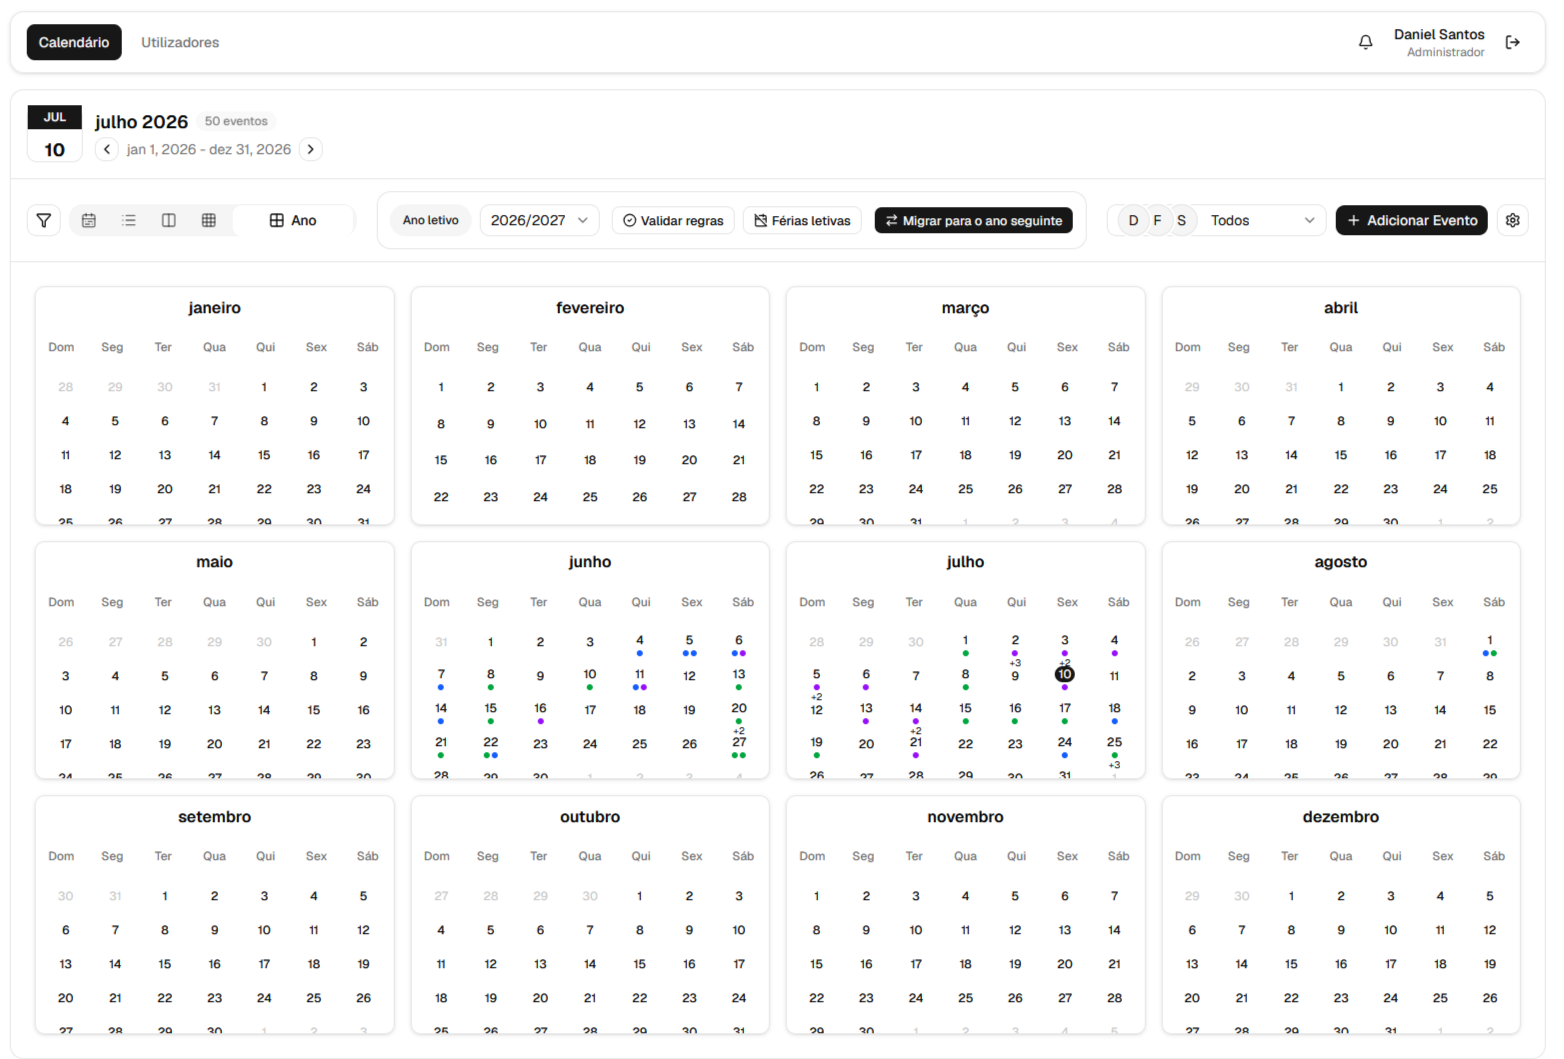
\includegraphics{./figures/app_screenshots/calendar_View_year.png}}
\end{center}
\caption{Calendar interface, Year view: a full-year grid overview of the academic calendar.}\label{fig:calendar-year}
\end{figure}

\clearpage
\section{Validation/Migration Results Modal} \label{app:migration-report}

Referenced from Section~\ref{sec:frontend-academic-year-tools}.

\begin{figure}[htbp]
\begin{center}
\resizebox{!}{160mm}{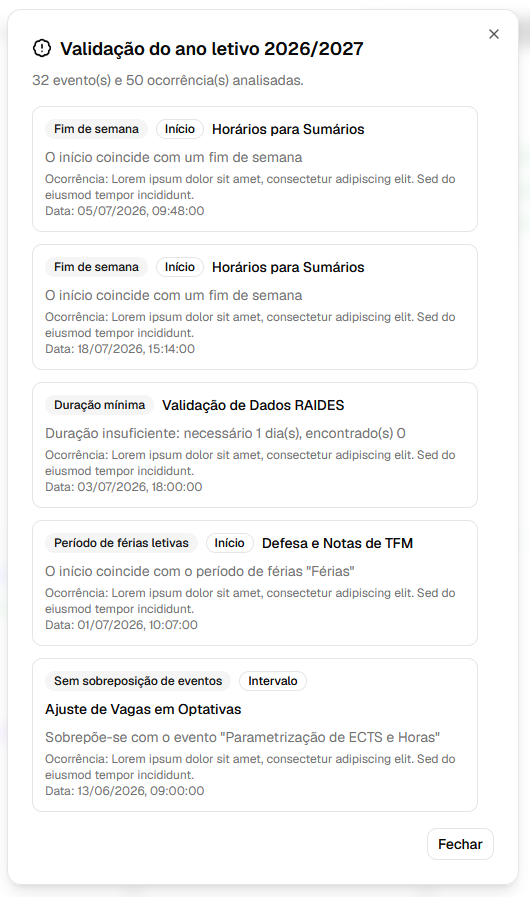
\includegraphics{./figures/app_screenshots/rules_validate.png}}
\end{center}
\caption{Validation/migration results modal: a confirmation banner when no rule violations are found, or one card per violation, each naming the rule, the affected event/occurrence, and the offending date.}\label{fig:migration-report-full}
\end{figure}
